% !TeX program = pdflatex
\documentclass[tikz,border=8pt]{standalone}
\usepackage{tikz}
\usetikzlibrary{angles,quotes,calc}
\definecolor{FigureBlue}{HTML}{2563EB}\definecolor{FigureOrange}{HTML}{EA580C}
\begin{document}
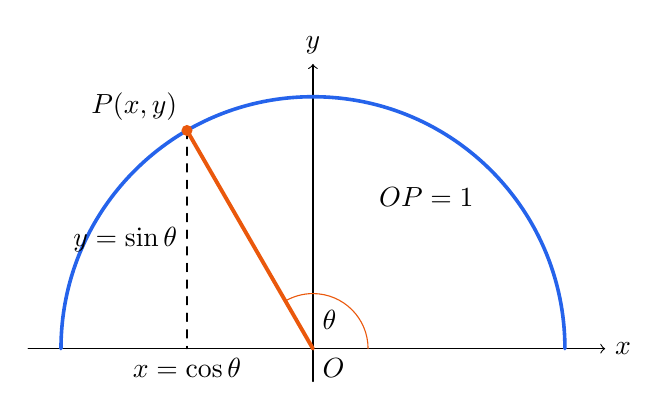
\begin{tikzpicture}[x=3.2cm,y=3.2cm,line cap=round]
  \coordinate (O) at (0,0); \coordinate (X) at (1,0); \coordinate (P) at (120:1); \coordinate (H) at (-.5,0);
  \draw[->] (-1.13,0)--(1.16,0) node[right] {$x$}; \draw[->] (0,-.13)--(0,1.13) node[above] {$y$};
  \draw[FigureBlue,line width=1.3pt] (1,0) arc[start angle=0,end angle=180,radius=1];
  \draw[FigureOrange,line width=1.4pt] (O)--(P); \draw[dashed] (P)--(H);
  \pic[draw=FigureOrange,angle radius=7mm,"$\theta$"] {angle=X--O--P};
  \fill[FigureOrange] (P) circle (2pt); \node[above left] at (P) {$P(x,y)$};
  \node[below] at (H) {$x=\cos\theta$}; \node[left] at ($(P)!.5!(H)$) {$y=\sin\theta$};
  \node[below right] at (O) {$O$}; \node at (.45,.6) {$OP=1$};
\end{tikzpicture}
\end{document}
